% v2-acmsmall-sample.tex, dated March 6 2012
% This is a sample file for ACM small trim journals
%
% Compilation using 'acmsmall.cls' - version 1.3 (March 2012), Aptara Inc.
% (c) 2010 Association for Computing Machinery (ACM)
%
% Questions/Suggestions/Feedback should be addressed to => "acmtexsupport@aptaracorp.com".
% Users can also go through the FAQs available on the journal's submission webpage.
%
% Steps to compile: latex, bibtex, latex latex
%
% For tracking purposes => this is v1.3 - March 2012

\documentclass[prodmode,acmtecs]{acmsmall} % Aptara syntax

\usepackage{graphicx}
\usepackage{caption}
\usepackage{subfigure}
\usepackage{setspace}
\usepackage{tabulary}
\usepackage{lineno}
\usepackage{xfrac}

\usepackage{alltt}
\renewcommand{\ttdefault}{txtt}

\usepackage{listings}
\lstset{language=C, breaklines=true}

\usepackage[cmex10]{amsmath}
\usepackage{url}

% Package to generate and customize Algorithm as per ACM style
\usepackage[ruled]{algorithm2e}
\renewcommand{\algorithmcfname}{ALGORITHM}
\SetAlFnt{\small}
\SetAlCapFnt{\small}
\SetAlCapNameFnt{\small}
\SetAlCapHSkip{0pt}
\IncMargin{-\parindent}

% Metadata Information
%\acmVolume{9}
%\acmNumber{4}
%\acmArticle{39}
%\acmYear{2010}
%\acmMonth{3}

% Document starts
\begin{document}

% Page heads
\markboth{F. Luporini et al.}{Optimizing Finite Element Integration through Automated Expression Rewriting and Code Specialization}

% Title portion
\title{Optimizing Finite Element Integration through Automated Expression Rewriting and Code Specialization}
\author{Fabio Luporini
\affil{Imperial College London}
David A. Ham
\affil{Imperial College London}
Paul H.J. Kelly
\affil{Imperial College London}}
% NOTE! Affiliations placed here should be for the institution where the
%       BULK of the research was done. If the author has gone to a new
%       institution, before publication, the (above) affiliation should NOT be changed.
%       The authors 'current' address may be given in the "Author's addresses:" block (below).
%       So for example, Mr. Abdelzaher, the bulk of the research was done at UIUC, and he is
%       currently affiliated with NASA.

\begin{abstract}
Abstract goes here
%
%The code is generated from a high level language for PDEs. An
%invocation of the kernel typically does tensor-like calculators over
%relatively small matrices; e.g., triply nested loops operating on
%about a dozen iterations. Because of the DSL context, COFFEE has a lot
%of flexibility on how it organizes/orders the calculations to tailor
%execution to a target architecture.
%
\end{abstract}

\category{G.1.8}{Numerical Analysis}{Partial Differential Equations -
  Finite element methods}

\category{G.4}{Mathematical Software}{Parallel and vector
  implementations}

\terms{Design, Performance}

\keywords{Finite element integration, local assembly, compilers,
  optimizations, SIMD vectorization}

\acmformat{Fabio Luporini, David A. Ham, and Paul   H. J. Kelly, 2014. 
  Optimizing Finite Element Integration through Automated Expression Rewriting and Code Specialization.}

% At a minimum you need to supply the author names, year and a title.
% IMPORTANT: Full first names whenever they are known, surname last,
% followed by a period.  In the case of two authors, 'and' is placed
% between them.  In the case of three or more authors, the serial
% comma is used, that is, all author names except the last one but
% including the penultimate author's name are followed by a comma, and
% then 'and' is placed before the final author's name.  If only first
% and middle initials are known, then each initial is followed by a
% period and they are separated by a space.  The remaining information
% (journal title, volume, article number, date, etc.) is
% 'auto-generated'.

\begin{bottomstuff}

This research is partly funded by the MAPDES project, by the
Department of Computing at Imperial College London, by EPSRC through
grants EP/I00677X/1, EP/I006761/1, and EP/L000407/1, by NERC grants
NE/K008951/1 and NE/K006789/1, by the U.S.  National Science
Foundation through grants 0811457 and 0926687, by the U.S. Army
through contract W911NF-10-1-000, and by a HiPEAC collaboration
grant. The authors would like to thank Dr. Carlo Bertolli,
Dr. Lawrence Mitchell, and Dr. Francis Russell for their invaluable
suggestions and their contribution to the Firedrake project.

Author's addresses: Fabio Luporini $\&$ Paul H. J. Kelly, Department of Computing,
Imperial College London; David A. Ham, Department of Computing and
Department of Mathematics, Imperial College London; 
\end{bottomstuff}

\maketitle

%Computational cost is a critical limitation in scientific computing,
%especially for finite element simulations. To provide one particular
%example we are particularly concerned about, it has been well
%established that mesh resolution Consequently, our aggressive
%optimization of local assembly, which may even take up to 60% of the
%overall FEM's execution time, directly impacts the performance of
%large-scale scientific simulations running on supercomputers.

\section{Introduction}

%This paper can be thought of as a continuation of the work presented in~\cite{Luporini}: in particular, we answer the remaining open questions, generalize and formalize an approach to minimize redundant computation using a similar philosophy, we show ~\cite{quadrature1}. 


\section{Preliminaries}
\label{sec:background}

\subsection{Quadrature for Finite Element Local Assembly}
%Here we discuss about the computational characteristics of
%computational science kernels. Briefly cite op2 kernels. Emphasis on
%Finite Element Assembly. Generalization and formalization of a Finite
%Element Assembly kernel using quadrature representation.

% ASSEMBLY EXPRESSION == THE EXPRE// COMPUTATION OF ELEMENT MATRIX

\subsection{Code Generation for Quadrature Representation}
Rapid implementation of high performance, robust, and portable code evaluating element matrices using quadrature can be achieved through automated code generation. This has been succesfully proved in the context of the popular FEniCS project~\cite{Fenics}. The FEniCS Form Compiler (FFC) accepts as input the variational form of a partial differential equation and generates C++ code implementing local assembly routines. The variational form is expressed at high-level by means of the domain-specific Unified Form Language (UFL). Local assembly code must be high performance: as the complexity of a form increases, in terms of number of derivatives, pre-multiplying functions, and polynomial order of the chosen functions, the resulting kernels evaluating element matrices become more computationally expensive, which impacts significantly the run-time of the overall computation. 

Achieving high performance is non-trivial due to the complexity of the mathematical expressions involved in the numerical integration and because of the small sizes of loops and accessed arrays. In~\cite{quadrature1},~\cite{Kirby-FEM-opt} and~\cite{Francis}, it is shown how automated code generation allows the introduction of powerful optimizations, which a user cannot be expected to write ``by hand'', as well as the exploration of non-standard integration techniques, based, for instance, on symbolic manipulation. In~\cite{Luporini} we made one step forward by showing that different problems require distinct set of transformations if close-to-peak performance needs to be obtained, and that low-level, domain-aware code transformations, which are not supported by available compilers, are essential to maximize instruction-level parallelism and register locality. 

\subsection{Summary of Low-level Optimizations for Quadrature Representation}
\label{sec:summary-opts}
To neatly distinguish the contributions of this paper from those in~\cite{Luporini}, in this section we summarize the results of our previous work on automated code transformations for quadrature representation.

...TODO...

The work in~\cite{Luporini} resulted in the development of COFFEE\footnote{COFFEE stands for COmpiler For FinitE Element local assembly.}, a compiler for the optimization of local assembly kernels relying on quadrature representation.  

...TODO...

Temporary arrays can be placed at the right depth in the sorrounding loop nest to store values of sub-expressions that are invariant to one or more loops. 

...TODO...

% Far notare che low-level si, ma sono guidate da high-level knowledge! Questo in risposta alla domanda: ma allora perche' non sfruttare la domain knowledge che hai, che senso ha separare...

% Ci sono due goal: minimizzare flops e specializzare

% Vantaggio di automatizzare rispetto che scrivere a mano
% which would be practically unfeasible to achieve by hand-written code


\section{A Compiler for Optimizing Quadrature-based Integration}
In order to generate high performance code, mathematical expressions evaluating the element tensor must be optimized with regards to several interrelated aspects: 1) minimization of floating point operations, 2) instruction-level parallelism, and 3) data locality. In this paper, we tackle these three points building on our previous work (\cite{Luporini}). 

...We propose a novel structure of how we think a platform-independent, domain-specific optimizing compiler should look like....

\begin{figure}
\begin{center}
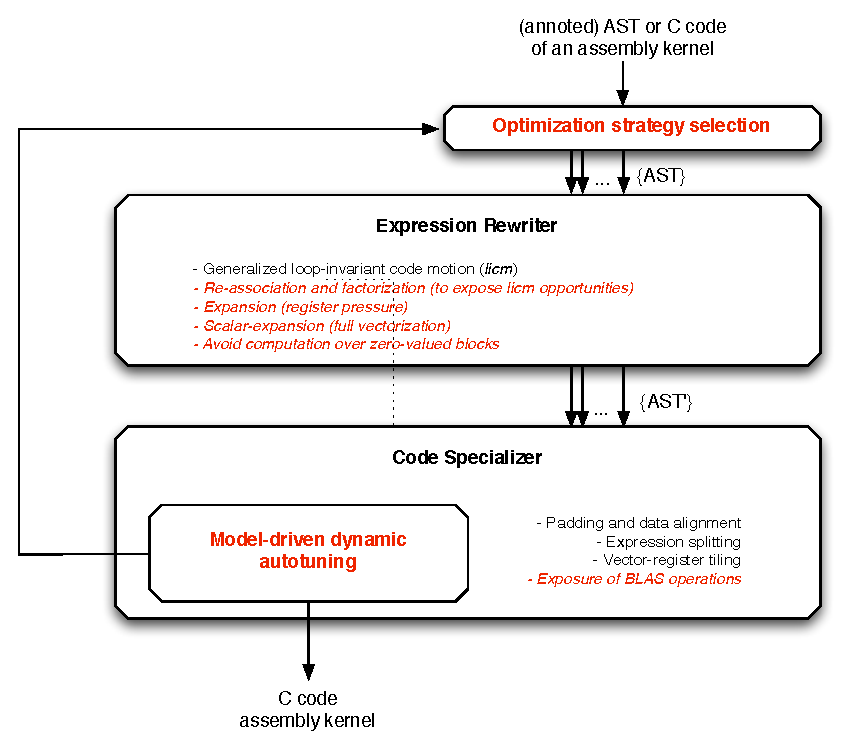
\includegraphics[scale=0.6]{pictures/coffee-scheme}
\caption{Outline of COFFEE}\label{fig:coffee-outline}
\end{center}
\end{figure}


The high-level structure of COFFEE is shown in Figure~\ref{fig:coffee-outline}. 

...The Expression Rewriter is a software module implemented in COFFEE dealing with the first point...

...The Code Specializer (henceforth CS) is...
A key point is that the ER has to perform transformations that do not break the code specializer. Having indirections is really dangerous...


\section{Expression Rewriting}
\label{sec:expr-rewriting}
As summarized in~\ref{sec:summary-opts}, loop-invariant code motion is the key to reduce the computational intensity of a mathematical expression. The Expression Rewriter (henceforth ER) that we have designed and implemented in COFFEE enhances this technique by making two steps forward, which allow more redundant computation to be avoided. 

Firstly, exploiting arithmetic operations properties like associativity, distributivity, and commutativity, it manipulates the original expression to expose more opportunities to the code hoister. There are many possibilities of rewriting an expression, and the search space can quickly become too big. Therefore, one problem we solve is finding a sufficiently simple yet systematic way of maximizing the amount of loop-invariant operations in an expression. In Section~\ref{sec:rewriting-rules}, we formalize the set of rewrite rules that COFFEE follows to transform an expression. 

Secondly, the ER re-structures the loop nest so as to eliminate arithmetic operations over array columns that are statically known to be zero-valued. Zero columns in tabulated basis functions appear, for example, when taking derivatives on a reference element or when using mixed elements. A code transformation eliminating floating point operations on zeros was presented in~\cite{quadrature1}; however, the issue with it is that by using indirection arrays in the generated code, it breaks many of the optimizations that can be applied at the Code Specializer level, including SIMD vectorization. In Section~\ref{sec:zeros}, we show a novel approach to avoiding computation on zeros based on symbolic execution.

%In COFFEE, the application of the re-writing rules preceds the elimination of operations on zeros. 

%It is worth noting how writing these transformations ``by hand'' would be practically unfeasible, especially when the expressions are particularly complex.
%
%
%In this section, we describe our efforts in producing a more effective tool capable of explore how to leverage automated code generation to expose more opportunities to the code hoister. 
%
%Automated code generation, however, Mathematical expressions can be transformed to decrease the number of arithmetic operations required to evaluate the element tensor. A first 
%
%Minimizing the number of floating point operations for evaluating the element tensor of a generic form
%

\subsection{Objectives of the Expression Rewriter}
\label{sec:rewriting-rules}

\begin{figure}
\tiny
\lstinputlisting{listings/simple.code}
\caption{Original code}\label{fig:original-code}
\end{figure}

Consider the simplified example of the element matrix computation in Figure~\ref{fig:original-code}, which is an excerpt from a real Burgers problem. In practice, depending on the problem, the expression tree could be much more complex, with multiple levels of nesting. The example is however representative for a large class of problems, so we will use it throughout the rest of the paper for illustrative purpose. 

A first glimpse of the code suggests that the sub-expression \texttt{F[i][j]*d + G[i][j]*e} is invariant with respect to the innermost loop, so it should be hoisted at the level of the outer loop \texttt{j}. This is a standard compiler transformation, which is supported by any available compilers. With a closer look we notice that the sub-expression \texttt{a*C[i][k] + b*E[i][k]} is also invariant, although, in this case, with respect to the outer loop \texttt{j}. In~\cite{Luporini}, we have showed that a \textit{generalized} loop-invariant code motion transformation - that is, given a non-trivial expression, the capability of analyzing all of its sub-expressions with respect to the enclosing loops to determine what code is hoistable- is not supported by available compilers. Moreover, the lack of cost models to ascertain both the optimal place where to hoist an expression and whether or not vectorizing it at the price of extra temporary memory is a fundamental limiting factor. We have addressed these problems by implementing a generalized loop-invariant code motion transformation in COFFEE.

We now consider the case of forms that ``hide'' further opportunities for code hoisting. Such forms are by no means exotic: for example, the pattern described next is commonly found in elastic problems. By examining again the example in Figure~\ref{fig:original-code}, we notice that the basis function array \texttt{B}, iterating along the iteration space \texttt{[i,j]}, appears twice in the expression. If we expand the products in which \texttt{B} is accessed, we can apply product commutativity and then factorize the expression as in Figure~\ref{fig:factorized-code}. This has two effects: firstly, it reduces the total number of arithmetic operations performed; secondly, and most importantly, it exposes a new sub-expression \texttt{(A[i][k]/c + T2[k]*f)} invariant with respect to loop \texttt{j}. Therefore, code hoisting can be performed.

\begin{figure}
\tiny
\lstinputlisting{listings/factorized.code}
\caption{Factorized code}\label{fig:factorized-code}
\end{figure}

The second observation we make concerns the register pressure induced by the expression. Once loop-invariant terms are lifted, we can think about data locality and, in particular, register allocation. Assume the local assembly kernel is executed on a state-of-the-art architecture having 16 logical registers, e.g. an Intel Haswell. Each value appearing in the expression is loaded and kept in a register as long as possible. For instance, the scalar value \texttt{g} is loaded once, whereas the term \texttt{det*W[i]} is precomputed and loaded in a register at every $i$ iteration. This implies that at every iteration of the \texttt{jk} loop nest, 12$\%$ of the available registers are spent just to store constant values. In more complicated expressions, the percentage of registers destined to store loop-invariant terms can be even higher. Registers are, however, a precious resource, especially when evaluating intensive expressions. The smaller is the number of free registers, the worse is the instruction-level parallelism achieved: for example, a shortage of registers can increase the pressure on the L1 cache (i.e. it can worsen data locality), or it may prevent the effective application of standard transformations like loop unrolling. The ER works around this problem by suitably expanding terms and introducing, where necessary, new temporary values. 

%An analogous analysis applies to processors with larger numbers of registers, since using loop unroll or loop unroll-and-jam to expose more instruction-level parallelism would increase the requirements on registers.

\begin{figure}
\tiny
\lstinputlisting{listings/toexpand.code}
\caption{Expandable code}\label{fig:toexpand-code}
\end{figure}

Consider the variant of the running (transformed) example shown in Figure~\ref{fig:toexpand-code}. Again, this is a representative example of what happens in real finite element forms. We can easily distribute \texttt{det*W[i]} over the three operands on the left-hand side of the multiplication, and then absorb it in the pre-computation of \texttt{T1}, resulting in the code illustrated in Figure~\ref{fig:expanded-1-code}. Freeing the register destined to the constant \texttt{g} is more complicated: we cannot absorb it in the pre-computation of \texttt{T1} because the same array is accessed in the evaluation of \texttt{(T1[ j]*A[i][k])}. The solution is to add another temporary as in Figure~\ref{fig:expanded-2-code}. Generalizing, this is a problem of data dependencies; in order to solve it, we employ a dependency graph in which we add a direct edge from identifier \texttt{A} to identifier \texttt{B} to denote that the evaluation of \texttt{B} depends on \texttt{A}. The dependency graph is initially empty; every time a new temporary is created due to loop-invariant code motion or expansion of terms is performed, it is updated by suitably adding vertices and edges.

\begin{figure}[t]
\tiny
\centering     
\subfigure[Expanded 1 code]{\label{fig:expanded-1-code}\lstinputlisting{listings/expanded-1.code}}
~~
\subfigure[Expanded 2 code]{\label{fig:expanded-2-code}\lstinputlisting{listings/expanded-2.code}}
\caption{Expanded code.}\label{fig:expanded-code}
\end{figure}

\subsection{Rewrite Rules}
In general, assembly expressions produced by automated code generation can be much more complex (more terms and operations involved) and nested. Our goal is to establish a portable, platform- and compiler-independent, and systematic way of reducing the strength of an expression. The technique should be simple; definitely it must be robust to be integrated in an optimizing domain-specific compiler capable of supporting real problems. Ideally, it should be naturally extendible to problems that will be supported in next releases of state-of-the-art frameworks like Firedrake and FEniCS: for instance, explicit support for outer-product finite elements will enable generation of kernels with much deeper loop nests, and the ER should transparently be able to deal with these structures as well. 

To address these issues, we have based the implementation of the ER in COFFEE on a set of formal rewrite rules. By applying these rules, it is possible to derive how an expression will be transformed, as well as what and where (i.e. at which level in the loop nest) temporaries will be introduced. When applying a rule, the ER needs to update the state of the loop nest, to reflect, for example, the use of a new temporary and the newly created data dependencies. We define, therefore, the state of a loop nest $L = (\sigma, G)$, where $G = (V, E)$ represents the dependency graph, while $\sigma$ maps invariant sub-expressions to identifiers of temporary arrays. We also introduce the \textit{conditional hoister} operator $[]$ on $\sigma : Inv \rightarrow S$ such that
\begin{gather*}
\sigma[\sfrac{v}{x}] = 
\begin{cases}
\sigma(x) \text{~~~~~~~~if $x \in Inv$; $v$ is ignored}\\
v \text{~~~~~~~~~~~~~if $x$ $\notin$ $Inv$; $\sigma$(x) = v}\\
\end{cases}
\end{gather*}
That is, intuitively, if the invariant expression \texttt{x} has already been hoisted, then return the temporary identifiers that hosts its value; otherwise, hoist the expression. There is a special case when $v = \perp$, used to delete entries in $\sigma$. Specifically:
\begin{gather*}
\sigma[\sfrac{\perp}{x}] = 
\begin{cases}
\sigma(x) \text{~~~~~~~~if $x \in Inv$; $\sigma = \sigma \setminus (x, \sigma(x))$}\\
t \text{~~~~~~~~~~~~~~if $x$ $\notin$ $Inv$; $t \notin Inv$}\\
\end{cases}
\end{gather*}
In other words, the previously hoisted expression \texttt{x} is removed (if any) and the temporary identifier that was hosting its value is returned. This is useful to express updates of invariant expressions.
Rewrite rules for the ER are provided in Figure~\ref{fig:rewrite-rules}; obvious rules are omitted for brevity. Conceptually, the ER visits the expression tree from the root, which is the outermost operation, and applies the transformations dictated by the rewrite rules. As an example, one can try instantiating the rules in the code of Figures~\ref{fig:original-code} and~\ref{fig:toexpand-code}; eventually, the optimized code in Figures~\ref{fig:factorized-code} and~\ref{fig:expanded-2-code} is obtained, respectively. 

\begin{figure}
\small
\centering
\begin{spacing}{1.5}
\begin{align*}
[a_i \cdot b_j]_{(\sigma, G)} &\rightarrow [a_i \cdot b_j]_{(\sigma, G)} ~~&~~&\\
[(a_i + b_j)\cdot \alpha]_{(\sigma, G)} &\rightarrow [(a_i \cdot \alpha + b_j \cdot \alpha)]_{(\sigma, G)} ~~&~~ &\\
[a_i \cdot b_j + a_i \cdot c_j]_{(\sigma, G)} &\rightarrow [(a_i \cdot (b_j + c_j)]_{(\sigma, G)} ~~&~~ &\\
[a_i + b_i]_{(\sigma, G)} &\rightarrow [t_i]_{(\sigma', G')} ~~&~~ &t_i = \sigma[\sfrac{t_i'}{a_i + b_i}], G' = (V \cup {t_i}, E \cup \lbrace(t_i, a_i), (t_i, b_i)\rbrace)\\
[(a_i \cdot b_j) \cdot \alpha]_{(\sigma, G)} &\rightarrow [t_i \cdot b_j]_{(\sigma', G')} ~~&~~ &\sharp(b_j) > \sharp(a_i), t_i = \sigma[\sfrac{\sigma[\sfrac{\perp}{a_i}]}{a_i \cdot \alpha}], a_i \notin in(G), \\
~&~~&~~&G' = (V \cup {t_i}, E \cup \lbrace(t_i, a_i), (t_i, \alpha)\rbrace)\\
[(a_i \cdot b_j) \cdot \alpha]_{(\sigma, G)} &\rightarrow [t_i \cdot b_j]_{(\sigma', G')} ~~&~~ &\sharp(b_j) > \sharp(a_i), t_i = \sigma[\sfrac{t_i'}{a_i \cdot \alpha}], a_i \in in(G), \\
~&~~&~~&G' = (V \cup {t_i}, E \cup \lbrace(t_i, a_i), (t_i, \alpha)\rbrace)\\
\end{align*}
\end{spacing}
\caption{Rewrite rules.}\label{fig:rewrite-rules}
\end{figure}
 
%TODO: each level in sigma is then taken and wrapped in a loop 
 
% blablabla molto complesse, nestings etc expose etc allora rewrite rules 

% we will show the effects of this stuff over plain LICM in section


% hoisting constants release registers!!!!

\subsection{Avoiding Iteration on Zero-blocks by Symbolic Execution}
\label{sec:zeros}
The second task of the ER consists of skipping arithmetic operations over blocks of zero-valued entries in basis function and derivatives of basis functions arrays. Zero columns in such arrays arise, for example, when taking derivatives on a reference element and when employing mixed elements. In~\cite{quadrature1}, a code transformation to eliminate floating point operations on zero columns was introduced; the technique was implemented in FEniCS. We will evaluate our approach and compare it to this pioneering work in Section~\ref{sec:perf-results}. We propose a strategy in which we avoid the use of indirection arrays in the generated code (e.g. \texttt{A[B[i]]}, where \texttt{A} is a tabulated basis function and \texttt{B} a map from loop iterations to non-zero columns in \texttt{A}), which otherwise would break the optimizations applicable at the Code Specializer level, especially SIMD vectorization. 

\begin{figure}[t]
\tiny
\centering     
\subfigure[Factorized, showing zeros, code]{\label{fig:withzeros-code}\lstinputlisting{listings/withzeros.code}}
~~~~~~~~~~~~~~~~~~~~~~~~~~~~~~~~~~~~~~~~~~
\subfigure[Factorized, skipping zeros, code]{\label{fig:withzeros-skipped-code}\lstinputlisting{listings/skipzeros.code}}
\caption{Without and with skipping zeros}\label{fig:skip-code}
\end{figure}

Consider Figure~\ref{fig:withzeros-code}, which is an enriched version of the transformed Burgers excerpt in Figure~\ref{fig:factorized-code}. The code is instantiated for the specific case of polynomial order 1, Lagrange elements on a 2D mesh. The array \texttt{D} represents a tabulated derivative of a basis function at the various quadrature points. We notice the presence of 4 zero-columns. Any multiplications or additions along these columns could (should) be skipped in order to minimize irrelevant floating point operations. One solution, as anticipated, is not to generate the zero columns, i.e. to generate a dense 6$\times$2 array, to reduce the size of the iteration space over test and trial functions (from 6 to 2), and to use an indirection array (e.g. $ind = \lbrace 3, 5\rbrace$) to access the right entries in the element tensor $A$. As explained, this prevents, among the various optimizations, effective code vectorizability, because memory loads and store would eventually reference non-contiguous locations. 
%on the other hand, reshrinki tutto su un array solo...

Our approach is based on domain knowledge and symbolic execution. We discern the origin of zero-columns: for example, those due to taking derivatives on the reference element from those inherent to using mixed (vector) elements. In the running Burgers example, the use of vector function spaces require the generation of a zero-block (columns 0, 1, 2 in the array \texttt{D}) to preserve the correctness of the element matrix evaluation while iterating along the space of test and trial functions. The two key observations are that 1) the number of zero-columns caused by mixed elements is much larger then that due to derivatives, and 2) such columns are contiguous in memory. Based on this, we decide to skip any computation involving zero-columns induced by mixed elements, whereas we still iterate over any other zero-columns. Consequently, the only modifications to the code that are eventually needed are adjusting loop bounds and introducing offsets when accessing the element matrix, as shown in Figure~\ref{fig:withzeros-skipped-code}. In general, multiple iteration spaces over test and trial functions (i.e. \texttt{jk} loops), characterized by their own loop bounds, may be needed, increasing loop overhead and decreasing data locality for the element matrix.

The implementation is based on symbolic execution. The ER expects information from the higher layer about where the zero-blocks are located, in each tabulated basis function. This could come in the form of code annotation if the input to COFFEE were provided as a C string (as shown in Figure~\ref{fig:withzeros-skipped-code}) or by suitably decorating basis functions nodes in the abstract syntax tree representing the local assembly routine. Then, each statement in the local assembly loop nest is symbolically executed. For example, consider the statement \texttt{T2[r] = ((d*D[i][k])+(e*E[i][k]));} in Figure~\ref{fig:withzeros-skipped-code}. Array \texttt{D} has non-zeros in positions $NZ_D = [3,5]$; we also assume \texttt{E} has non-zeros in positions $NZ_E = [0,2]$. Multiplications by scalar do not affect the propagation of zero columns. On the other hand, when summing the two operands \texttt{d*D[i][k]} and \texttt{e*E[i][k]}, we record that the target identifier \texttt{T2} will have non-zero columns in positions $NZ_D \cup NZ_E = [0-5]$. Exploiting the $NZ$ information associated with each identifier, the assembly expression is split into several sets of sub-expressions, each set characterized by accesses to the same range of non-zero columns and, therefore, iterating over a suitably-sized iteration space. In our example, there is just one set, which contains two sub-expressions, enclosed in a doubly nested loop of size 3$\times$3.

...TODO...: dire come si riaggiustano gli indici quando si vuole usare AVX ma la parte dense non e' multiplo del vector length - se non e' paddata la tail, allora si decrementa lo starting index di un pochino, tanto sono zeri...

\section{Code Specialization}
\label{sec:code-spec}
The Code Specializer is the second software component of COFFEE. It provides a range of code transformations tailored for optimizing instruction-level parallelism and register locality. As summarized in Section~\ref{sec:summary-opts} and described in~\cite{Luporini}, padding and data alignment, expression splitting, and outer-product vectorization, which is a domain-aware implementation of vector-register tiling, are examples of optimizations that the Code Specializer is capable of applying. In this paper, we enrich this set of transformations as detailed in the following sections.

\subsection{Vector-expansion of Invariant Terms}
\label{sec:vect-exp}
The Expression Rewriter's loop-invariant code motion hoists invariant sub-expressions in the body of the outermost loop along which they iterate. If such a sub-expression computes a value depending on the outermost loop only, then the only way of vectorizing it -- if we exclude superword level parallelism~\cite{SLP}, which is in general not applicable to our kernels -- is by vector-expansion of terms. 

\begin{figure}[t]
\tiny
\centering     
\subfigure[To vector expand code]{\label{fig:tovectexpand-code}\lstinputlisting{listings/tovectexpand.code}}
~~~~~~~~~~~~~~~~~~~~~~~~~~~~~~~~~~~~~~~~~~
\subfigure[Vector-expanded code]{\label{fig:vectexpanded-code}\lstinputlisting{listings/vectexpanded.code}}
\caption{Before and after vector expansion}\label{fig:skip-code}
\end{figure}

An example is given in Figure~\ref{fig:tovectexpand-code}: \texttt{F1, F2, F3, T1} are all scalar quantities, and their computation will not be auto-vectorized (as explained in Section~\ref{sec:perf-results}, we experimented with the Intel and GNU compilers). The argument that the cost of evaluating such expressions is not relevant because their computational cost is $O(I)$, while the evaluation of the element matrix has a cost of $O(I \cdot T^2)$, is too superficial, in general. There are notable cases, for instance problems based on hyperlasticity, for which the Expression Rewriter produces a significantly-large number of invariant scalar terms, which dramatically impact the execution time.

We have implemented a procedure that vector-expands scalar expressions, while lifting them outside of the loop nest as shown in Figure~\ref{fig:vectexpanded-code}. The dependency graph is queried to assess the legality of the transformation. At the price of extra memory, vector-expanded terms can now be vectorized by the compiler. 

% Expose vectorizability of the outermost loop 
% Render the loop nest perfect

\subsection{Exposing Linear Alegbra Operations}
In~\cite{Luporini}, we introduced the idea of transforming the element matrix evaluation into a sequence of calls to highly-optimized dense matrices multiply routines (henceforte DGEMM), for instance MKL or ATLAS BLAS. We compared COFFEE's optimizations with hand-written MKL-based kernels, showing how the small sizes of the involved arrays impair DGEMM calls. The study was conducted only in the case of a specific Helmholtz equation. There are cases, however, in which tabulated basis functions sizes grow up to a point for which certain BLAS implementations allow to achieve a better performance. For example, this may be the case of relatively-high polynomial orders or when the form is characterized by the presence of a number of pre-multiplying functions. To explore these extreme yet meaningful scenarios, we have developed an algorithm to reduce any generic element matrix evaluation to a sequence of DGEMM calls. 

The algorithm is shown in Figure~\ref{fig:algo-dgemm}. By using the rewrite rules in Figure~\ref{fig:rewrite-rules}, it can be proved that the Expression Rewriter can always reduce an assembly expression to a summation, over each quadrature point, of outer products along the test and trial functions. Each outer product is then isolated, i.e. the assembly expression is split into chunks, each chunk representing an outer product. Terms in the bodies of the various enclosing loops (e.g. coefficients evaluation at quadrature point, temporaries introduced by the Expression Rewriter) are vector-expanded and hoisted outside of the loop nest, as explained in Section~\ref{sec:vect-exp}. This implies that the loop nest is now perfect; that is, there is no intervening code among the various loops. The element matrix evaluation became a sequence of perfect loop nests, each loop nest computing a dense matrix-matrix multiply between temporaries hoisted by the Expression Rewriter or tabulated basis functions. Eventually, the storage layout of the involved operands is changed so as to be conforming to the BLAS interface (e.g. two dimensional arrays are flatten as one dimensional arrays). The translation of each loop nest into a DGEMM call is the last, straightforward step. 

% 
\subsection{Model-driven Dynamic Autotuning}
We have demonstrated in~\cite{Luporini} that there is no optimial set of code transformations. What sequence of transformations applying to a given problem depends on a broad range of factors, including mathematical structure of the input form, polynomial order of employed function spaces, presence of pre-multiplying functions, and, of course, the characteristics of the underlying architecture. COFFEE allows the user to abstract from finding the optimal combination of transformations for a given problem by resorting to its model-driven, dynamic autotuner. This is based on the idea that spending order of seconds to determine the fastest kernel implementation in a set of possible variants is a negligible overhead when it comes to iterate over real-life unstructured meshes, which can contain even up to trillions of elements~\cite{Rossinelli2013}.

In~\cite{Luporini}, we proposed a simple cost model that COFFEE could use to choose, given a problem, the transformations that were likely to maximize the performance. With this paper, however, we have added a significant number of options to the set of possible optimizations, which makes the selection problem far more challenging. The sole Expression Rewriter, for instance, could apply rewrite rules up to a number of pre-established depths, leading to the generation of many possible code variants.

We believe autotuning is an effective approach to tackling this problem. For each problem, not only does it allow to determine the best combination of transformations out of the set presented so far, also it enables exploring parametric low-level optimizations, such as loop unroll, unroll-and-jam, and interchange, by trying multiple unroll factors and loop permutations. By leveraging the cost model defined in our previous study, domain-awarness, and a set of heuristics, we manage to keep the autotuner overhead at a minimum, whilst achieving significant speed ups over purely cost-model-driven implementations. 



%1) dual approach to cost-model - more reliable? Easier...when zero-avoidance and low order, what is it best to do?
%2) self-building
%3) deeper exploration, to explore aggressive standard low-level transformations
%4) dynamic and heuristic-driven: 
%     - depending on kernel size, more or less unroll factors are used
%     - domain knowledge: no interchange test-trial functions loops
%     - no unroll innermost loop
%\subsection{Standard Compiler Transformations}



\section{Performance Evaluation}
\label{sec:perf-results}

\subsection{Experimental Setup}

%Experiments were run on a single core of two Intel architectures, a
%Sandy Bridge (I7-2600 CPU, running at 3.4GHz, 32KB L1 cache and 256KB
%L2 cache) and a Xeon Phi (5110P, running at 1.05Ghz in native mode,
%32KB L1 cache and 512KB L2 cache). We have chosen these two
%architectures because of the differences in the number of logical
%registers and SIMD lanes, which can impact the effectiveness of the
%optimization strategy. The \texttt{icc 13.1} compiler was used. On the
%Sandy Bridge, the compilation flags used were \texttt{-O2} and
%\texttt{-xAVX} for auto-vectorization. On the Xeon Phi, optimization
%level \texttt{-O3} was used. Other optimization levels performed, in
%general, slightly worse.

%\newcommand{\licmapresultsnorms}{
%\begin{tabulary}{1.0\textwidth}{cccccc|cccc}
%\cline{3-10}
%& & \multicolumn{4}{c}{\texttt{Sandy Bridge}} & \multicolumn{4}{c}{\texttt{Xeon Phi}} \\
%\cline{1-10}
%\texttt{problem} & \texttt{shape} & \texttt{p1} & \texttt{p2} & \texttt{p3} & \texttt{p4} & \texttt{p1} & \texttt{p2} & \texttt{p3} & \texttt{p4} \\[0.1cm]
%\texttt{Helmholtz} & \texttt{triangle} & 1.32 & 1.88 & 2.87 & 4.13 & 1,50 & 2,41 & 1,30 & 1,96 \\
%\texttt{Helmholtz} & \texttt{tetrahedron} & 1.35 & 3.32 & 2.66 & 3.27 & 1,41 & 1,50 & 2,79 & 2,81 \\
%\texttt{Helmholtz} & \texttt{prism} & 2.63 & 2.74 & 2.43 & 2.75 & 2,38 & 2,47 & 2,15 & 1,71\\[0.1cm]
%%\cline{1-18}
%\texttt{Diffusion} & \texttt{triangle} & 1.38 & 1.99 & 3.07 & 4.28 & 1,08 & 1,88 & 1,20 & 1,97\\
%\texttt{Diffusion} & \texttt{tetrahedron} & 1.41 & 3.70 & 3.18 & 3.82 & 1,05 & 1,51 & 2,76 & 3,00\\
%\texttt{Diffusion} & \texttt{prism} & 2.55 & 3.13 & 2.73 & 2.69 & 2,41 & 2,52 & 2,05 & 2,48\\[0.1cm]
%%\cline{1-18}
%\texttt{Burgers} & \texttt{triangle} & 1.56 & 2.28 & 2.61 & 2.77 & 2,84 & 2,26 & 3,96 & 4,27 \\
%\texttt{Burgers} & \texttt{tetrahedron} & 1.61 & 2.10 & 1.60 & 1.78 & 1,48 & 3,83 & 1,55 & 1,29 \\
%\texttt{Burgers} & \texttt{prism} & 2.19 & 2.32 & 1.64 & 1.42 & 2,18 & 2,82 & 1,24 & 1,25 \\
%\cline{1-10}
%\end{tabulary}
%}
%
%\begin{table*}[t]
%\tbl{Performance improvement due to generalized loop-invariant code
%  motion, data alignment, and padding, for different element shapes
%  (triangle, tetrahedron, prism) and polynomial orders ($p \in [1,
%    4]$), over the original non-optimized code, for the Helmholtz,
%  Diffusion and Burgers problems.}{ \scriptsize \licmapresultsnorms }
%\label{table:perf-results-licmap}
%\end{table*}

\subsection{Results for Forms of Increasing Complexity}

% Mass DGEMM utile explicit method etc

\section{Conclusions}
\label{sec:conclusions}


% Bibliography
\bibliographystyle{ACM-Reference-Format-Journals}
\bibliography{biblio}


\medskip

\end{document}
